%  !TeX  root  =  user_guide.tex

% when the revision of a section has been finalized,
% comment out the following line:
% \updatedisclaimer

\section{Расширение eVis}\label{sec:evis}

Управлением информатики биоразнообразия в Центре охраны природных ресурсов
и биоразнообразия Американского музея естественной истории \footnote{Раздел
взят из Руководства пользователя eVis (v1.1.0), Horning, N., K. Koy, P.
Ersts. 2009. Американский музей естественной истории, Центр охраны
биоразнообразия и природных ресурсов. Данный документ доступен по адресу
\url{http://biodiversityinformatics.amnh.org/}и выпущен под лицензией GNU FDL.}
было разработано расширение Event Visualization Tool (eVis),
программное обеспечение, расширяющее набор инструментов, используемых для
мониторинга окружающей среды и поддержки принятия решений в области,
связанной с охраняемыми природными территориями и ландшафтным планированием.
Данное расширение позволяет легко связывать геокодированные (то есть,
привязанные к координатам широты и долготы или X и Y) фотографии и прочие
документы поддерживаемых форматов с векторными данными в QGIS.

В новых версиях QGIS расширение eVis устанавливается и включается
автоматически. И по аналогии с остальными расширениями может быть
отключено или включено в Менеджере модулей QGIS (см. Раздел~\ref{sec:managing_plugins}).

В состав eVis входит три модуля: инструмент подключения к базе данных,
инструмент определения событий и обозреватель событий. Все эти модули
работают совместно, позволяя просматривать геокодированные фотографии
и прочие документы, связанные с объектами, хранящимися в векторных файлах,
базах данных и таблицах.

\subsection{Обозреватель событий}\label{evis_browser}

Модуль <<Обозреватель событий>> предназначен для отображения геокодированных
фотографий, ссылающихся на векторные объекты карты, открытой в QGIS. Например,
на точечные данные, загруженные в проект из векторного файла или в результате
запроса к базе данных. Такие векторные объекты должны содержать атрибутивную
информацию, описывающую местоположение, имя файла фотографии и (не
обязательно) направление компаса камеры в момент съёмки. Векторный слой
должен быть загружен в QGIS до запуска модуля <<Обозреватель событий>>.

\minisec{Запуск модуля <<Обозреватель событий>>}\label{evis_launch_browser}

Модуль <<Обозреватель событий>> можно запустить двумя способами:
нажав кнопку \\
\toolbtntwo{event_browser}{Обозреватель событий eVis} или
выбрав \mainmenuopt{Модули} \arrow \dropmenuopt{eVis} \arrow \\
\dropmenuopt{Обозреватель событий eVis}. Откроется окно \dialog{Обозреватель событий}.

В данном окне содержится три вкладки, расположенных сверху. Вкладка \tab{Вывод}
используется для просмотра фотографий и связанной с ними атрибутивной
информации. Вкладка \tab{Параметры} содержит набор настроек, позволяющих
управлять поведением расширения eVis. И, наконец, вкладка \tab{Внешние приложения}
используется для сопоставления расширений файлов, отличных от изображений,
и приложений, используемых в eVis для их отображения.

\minisec{Назначение окна Вывод}\label{evis_display_window}

Для просмотра окна Вывод щёлкните на вкладке \tab{Вывод} в
окне \dialog{Обозреватель событий}. Данное окно предназначено для просмотра
геокодированных фотографий и связанной с ними атрибутивной информации.

\begin{figure}[ht]
   \centering
   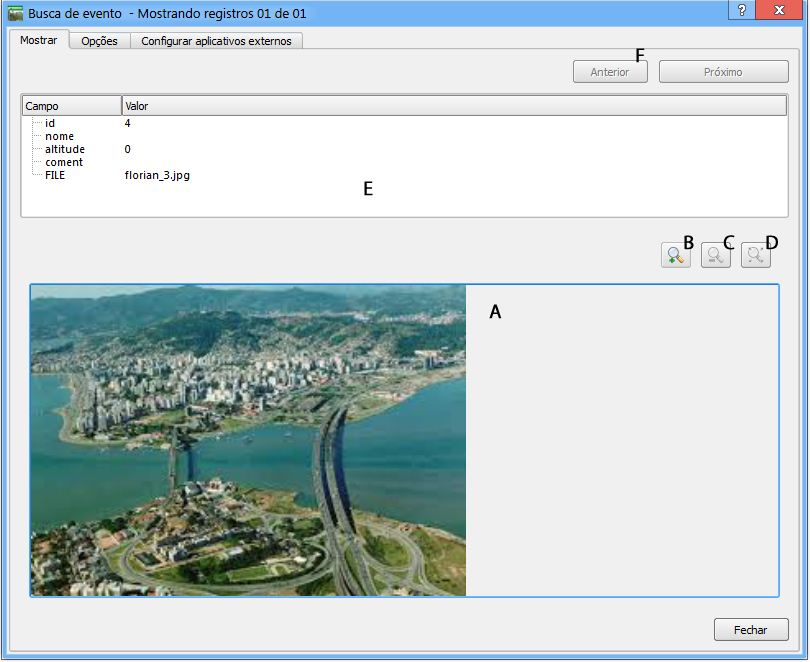
\includegraphics[clip=true, width=12cm]{evisdisplay}
   \caption{Окно Вывод расширения \emph{eVis} \wincaption}\label{evisdisplay}
\end{figure}

\begin{itemize}[label=--]
\item \textbf{Область вывода изображения}: Область отображения фотографий.
\item \textbf{Кнопка Увеличить}: Увеличьте фотографию для просмотра мелких
деталей. Если изображение полностью не помещается в окно просмотра,
воспользуйтесь полосами прокрутки, расположенными с левой и с нижней
стороны окна и позволяющими перемещаться по изображению.
\item \textbf{Кнопка Уменьшить}: Уменьшите фотографию для просмотра больших
территорий.
\item \textbf{Увеличить до полного охвата}: Отобразить полный охват
фотографии.
\item \textbf{Окно атрибутивной информации}: Вся атрибутивная информация
объекта, с которым связана фотография, представлена здесь. Если
файл, связанный с объектом, не является изображением, но его тип определён во
вкладке \tab{Внешние приложения}, то при двойном щелчке на значении поля,
содержащего путь до файла, запустится соответствующее приложение
для просмотра или прослушивания содержимого файла. Если тип файла определён,
то значение поля, содержащего путь до него, будет подсвечено зелёным цветом.
\item \textbf{Навигационные кнопки}: Если выделено более одного
объекта, то используйте кнопки \button{Предыдущее} и \button{Следующее}
для перехода между ними.
\item \textbf{Индикатор объектов}: Данный заголовок показывает, какой объект
в данный момент отображается и сколько ещё объектов доступно для отображения.
\end{itemize}

\minisec{Назначение окна Параметры}\label{evis_options_window}

\begin{figure}[ht]
   \centering
   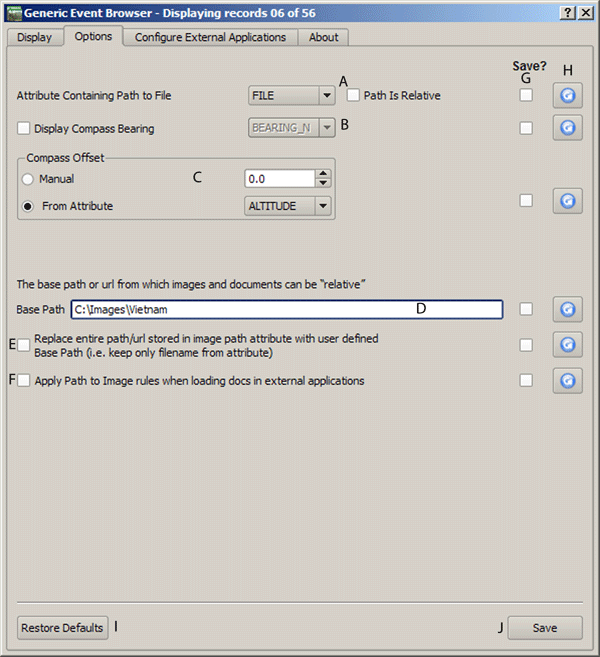
\includegraphics[clip=true, width=12cm]{evisoptions}
   \caption{Окно Параметры расширения \emph{eVis} \wincaption}\label{evisoptions}
\end{figure}

\begin{itemize}[label=--]
\item \textbf{Путь к файлу}: Выпадающий список для определения атрибутивного
поля, содержащего путь/URL фотографии или иного документа,
предназначенного для отображения. Если расположение представлено в виде
относительного пути, то должен быть отмечен соответствующий пункт.
Текстовое поле <<Базовый путь>> предназначено для определения базового пути до
файлов в случае использования относительных путей. Информация о
различных настройках расположения файлов представлена в Разделе~\ref{evis_specifying}.
\item \textbf{Магнитный азимут}: Выпадающий список для определения
атрибутивного поля, содержащего значение магнитного азимута, связанное с
отображаемой фотографией. Если значение магнитного азимута присутствует в
атрибутике слоя, то необходимо отметить пункт \checkbox{Показывать азимут}.
\item \textbf{Магнитное склонение}: Сдвиг компаса можно использовать для
компенсации магнитного склонения (позволяет адаптировать магнитные азимуты для
определения истинных географических). Отметьте пункт \radiobuttonon{{}Вручную},
чтобы задать значение сдвига компаса самостоятельно в соответствующем текстовом
поле или выберите пункт <<Из атрибута>> для определения поля, содержащего данное
значение. В обоих случаях для восточных склонений следует использовать
положительные величины, а для западных "--- отрицательные.
\item \textbf{Базовый путь}: Базовый путь, относительно которого определяются
относительные пути, определённые, как показано на Рисунке~\ref{evisoptions} (A).
\item \textbf{Полностью заменить путь на базовый}: Если отмечен этот пункт,
то из значения атрибута будет взято только имя файла и добавлено к базовому
пути.
\item \textbf{Применить правило ко всем документам}: Если отмечен данный
пункт, то все правила, относящиеся к настройке расположения изображений, будут
использованы и для других типов файлов, таких, как видео, текстовых документов и
звуковых файлов. Если данный пункт не отмечен, то все настройки расположения
файлов будут применены только к фотографиям, другие типы документов будут
игнорировать параметр <<Базовый путь>>.
\item \textbf{Сохранить параметр}: Если отмечен этот пункт, то
после закрытия окна или нажатия кнопки \button{Сохранить}, значение соответствующего
параметра будет сохранено для последующих сессий.
\item \textbf{Восстановить}: Сбросить и установить параметр в значение по
умолчанию.
\item \textbf{Восстановить по умолчанию}: Сбросить значения всех полей и
установить в значения по умолчанию. Данная операция эквивалентна
последовательному нажатию кнопок \button{Восстановить} возле каждого параметра.
\item \textbf{Сохранить}: Сохранить настройки, не закрывая вкладку
\tab{Параметры}.
\end{itemize}

\minisec{Назначение окна Внешние приложения}\label{evis_external_window}

\begin{figure}[htp]
   \centering
   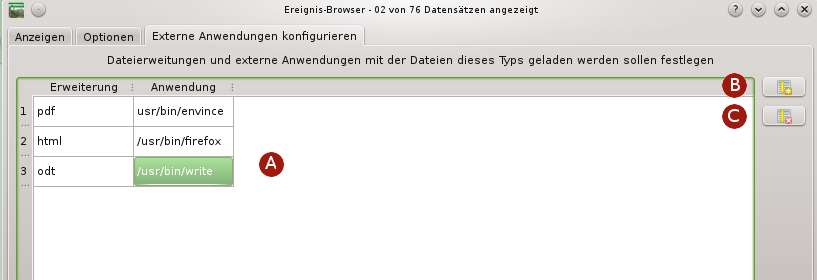
\includegraphics[clip=true, width=12cm]{evisexternal}
   \caption{Окно <<Внешние приложения>> расширения \emph{eVis} \wincaption}\label{evisexternal}
\end{figure}

\begin{itemize}[label=--]
\item \textbf{Таблица сопоставления}: Таблица содержит типы файлов, которые
можно открыть, используя eVis. Для каждого типа представляется расширение
и путь к приложению, позволяющему открыть файл данного типа. Таким образом,
появляется возможность открыть практически любой файл, например, видео,
звуковую запись или текстовый документ, а не только изображение.
\item \textbf{Добавить новый тип файлов}: Добавить новый тип файлов
с уникальным расширением и путь до приложения, которое его откроет.
\item \textbf{Удалить текущую строку}: Удалить из таблицы выбранный тип
файлов.
\end{itemize}

\minisec{Определение местоположения и названия фотографий}\label{evis_specifying}

Местоположение и название фотографий можно хранить, используя абсолютные или
относительные пути, или URL, если фотография хранится на Web-сервере.
Примеры различных подходов представлены в Таблице~\ref{tab:evis_examples}.

\begin{table}[htp]\index{модули!eVis}
\centering
\caption{Примеры записи адресов файлов с использованием абсолютных путей,
относительных путей и URL}\label{tab:evis_examples}\medskip
 \begin{tabular}{|p{0.50in}|p{0.50in}|p{5.0in}|p{0.7in}|}
 \hline \textbf{X} & \textbf{Y} & \textbf{FILE} & \textbf{BEARING}\\
 \hline 780596 & 1784017 & \filename{C:\textbackslash Workshop\textbackslash
eVis\_Data\textbackslash groundphotos\textbackslash DSC\_0168.JPG} & 275\\
 \hline 780596 & 1784017 & \filename{/groundphotos/DSC\_0169.JPG} & 80\\
 \hline 780819 & 1784015 &
\filename{http://biodiversityinformatics.amnh.org/evis\_test\_data/DSC\_0170.JPG} & 10\\
 \hline 780596 & 1784017 & \filename{pdf:http://www.testsite.com/attachments.php?attachment\_id-12}
& 76\\
 \hline
\end{tabular}
\end{table}

\minisec{Определение местоположения и названия прочих
документов поддерживаемых форматов}\label{evis_location}

Помимо фотографий, используя eVis, можно воспроизвести или просмотреть
текстовые документы, видео или звуковые файлы. Для этого в таблицу
сопоставления, расположенную во вкладке \tab{Внешние приложения} окна
\dialog{Обозреватель событий}, необходимо добавить сопоставление расширения
файла и приложения, с помощью которого этот файл можно будет открыть. Кроме
того, в таблице атрибутов векторного слоя должен присутствовать путь или URL
файла. При использовании URL следует соблюдать одно важное правило "--- URL
не должен содержать расширение файла, вместо этого расширение указывается
перед URL. Ссылка на файл будет иметь формат <<расширение:URL>>. То есть URL
предшествует расширение и двоеточие, что особенно удобно при осуществлении
доступа к документам Википедии и прочих Web-сайтов, в которых для управления
Web-страницами используются базы данных (смотри Таблицу~\ref{tab:evis_examples}).

\minisec{Использование Обозревателя событий}\label{evis_using_browser}

Если в атрибутике векторного слоя присутствует ссылка на фотографию и
информация о местоположении файла корректно установлена во вкладке
\tab{Параметры}, то после открытия окна \dialog{Обозреватель событий} должна
отобразиться фотография. Если фотография не появилась, то, возможно,
следует проверить настройки во вкладке \tab{Параметры}.

Если в таблице атрибутов слоя имеется ссылка на документ поддерживаемого
формата (или на изображение, имеющее расширение, не знакомое eVis), и во
вкладке \tab{Внешние приложения} описано приложение, открывающее файлы
данного типа, то поле, содержащее путь к файлу, будет выделено зелёным
цветом. Чтобы открыть документ, дважды щёлкните на этом поле. Если в
таблице атрибутов слоя имеется ссылка на документ, но путь к документу
не подсвечен зелёным цветом, то необходимо провести сопоставление расширения
и приложения во вкладке \tab{Внешние приложения}. Если путь подсвечен
зелёным, но по двойному нажатию документ не открывается, проверьте
настройки расположения файлов во вкладке \tab{Параметры}.

Если отображение азимута отключено во вкладке \tab{Параметры}, то векторный
объект, для которого открыта фотография, будет отмечен красной звёздочкой.
Если отображение азимута включено, то появится стрелка, указыающая в
направлении, соответствующем значению магнитного азимута. Стрелка будет
отцентрирована относительно объекта с которым связана фотография или иной объект.

Чтобы закрыть окно \dialog{Обозреватель событий}, нажмите кнопку \button{Закрыть}
во вкладке \tab{Вывод}.

\subsection{Определить события eVis}\label{evis_id_tool}

Модуль <<Определить события eVis>> позволяет отображать фотографии путём
щелчка на объектах карты, открытой в QGIS. Такие векторные объекты должны
содержать атрибутивную информацию, описывающую местоположение, имя файла
фотографии и (не обязательно) направление компаса камеры в момент съёмки.
Такой слой должен быть загружен в QGIS до запуска модуля определителя
событий.

\minisec{Запуск модуля Определить события}\label{evis_launch_id}

Для запуска модуля <<Определить события>> нажмите кнопку
\toolbtntwo{event_id}{Определить события eVis} или выберите
\mainmenuopt{Модули} \arrow \dropmenuopt{eVis} \arrow
\dropmenuopt{Определить события eVis}. После чего вид курсора изменится
на стрелку с символом <<i>>, что свидетельствует о том, что инструмент
определения события включён.

Для просмотра фотографий, связанных с объектами активного векторного слоя,
открытого в QGIS, поместите курсор на объект и щёлкните мышкой.
После щелчка на объекте откроется окно \dialog{Обозреватель событий} и
фотография, доступная для отображения в обозревателе, на месте щелчка
или около него. Если доступно несколько фотографий, то для перемещения между
различными объектами используйте кнопки \button{Предыдущее} и
\button{Следующее}. Остальные управляющие элементы описаны в разделе
<<Обозреватель событий>> данного руководства.

\subsection{Соединение с БД}\label{evis_database}

Модуль <<Соединение с БД>> представляет собой инструмент для соединения и
запросов к базам данных или иным ресурсам ODBC, таким, как электронные
таблицы.

eVis может напрямую соединяться с базами данных четырёх типов: Microsoft Access,
PostgreSQL, MySQL, SQLite, а также считывать данные через ODBC-соединения. При
считывании данных через ODBC-соединение (например, из электронных таблиц MS~Excel)
необходимо нужным образом сконфигурировать ODBC-драйвер в соответствии с типом
используемой операционной системы.

\minisec{Загрузка модуля соединения с БД}\label{evis_launch_database}

Для запуска модуля содинения с базой данных нажмите кнопку
\toolbtntwo{evis_connect}{Подключить базу данных eVis} или выберите \mainmenuopt{Модули} \arrow
\dropmenuopt{eVis} \arrow \dropmenuopt{Подключить базу данных eVis}.
После чего откроется окно \dialog{Соединение с БД}. Данное окно имеет
три вкладки: \tab{Предопределённые запросы}, \tab{Соединение с~БД} и
\tab{SQL-запрос}. Консоль вывода, расположенная внизу окна, отображает
статус действий, вызванных различными разделами данного модуля.

\minisec{Соединение с БД}\label{evis_connect_database}

Откройте вкладку \tab{Соединение с БД}, содержащую интерфейс подключения
к базе данных. Затем в выпадающем списке \dropmenuopt{Тип соединения}
выберите тип базы данных, к которой нужно подключиться. При необходимости
укажите имя пользователя и пароль в соответствующих полях Пользователь и
Пароль.

В соответствующем поле введите адрес сервера БД. Данная возможность
недоступна, если выбран тип базы данных <<MSAccess>>. Если база данных
размещается локально, то в качестве адреса следует указать <<localhost>>.

В поле <<База данных>> укажите имя базы данных. Если выбран тип <<ODBC>>, то
укажите здесь имя источника данных.

Когда все параметры заполнены, нажмите кнопку \button{Подключиться}. Если всё
прошло успешно, то в консоли вывода появится сообщение о том, что соединение
было установлено. Если соединение не было установлено, проверьте корректность
параметров, описанных выше.

\begin{figure}[ht]
   \centering
   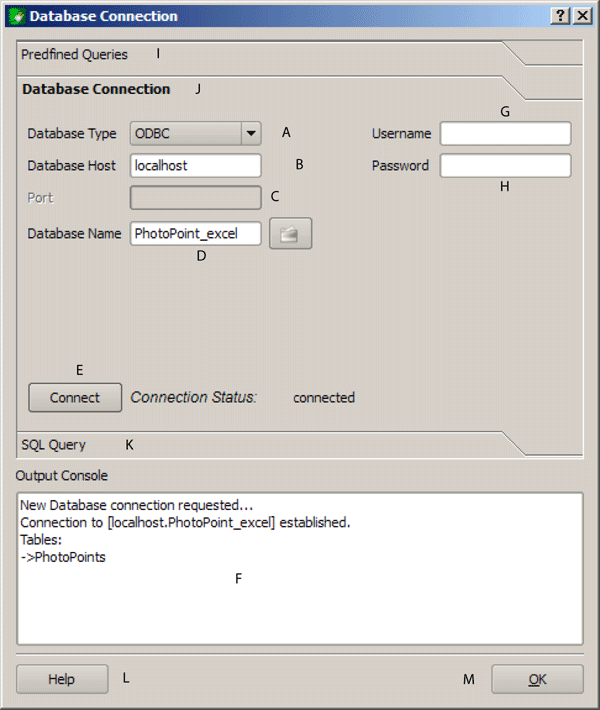
\includegraphics[clip=true, width=12cm]{evisdatabase}
   \caption{Окно <<Соединение с БД>> расширения \emph{eVis} \wincaption}\label{evisdatabase}
\end{figure}

\begin{itemize}[label=--]
\item \textbf{Тип соединения}: Выпадающий список, содержащий перечень
доступных типов баз данных.
\item \textbf{Сервер БД}: Адрес сервера баз данных.
\item \textbf{Порт} Номер порта в случае выбора базы данных MySQL или
PostgreSQL.
\item \textbf{База данных} Имя базы данных.
\item \textbf{Подключиться} Кнопка подключения к БД с использованием введёных
настроек.
\item \textbf{Консоль вывода} Консольное окно, в котором отображаются
сообщения, связанные с работой модуля.
\item \textbf{Пользователь}: Имя пользователя, указываемое в случае
защиты доступа к базе данных паролем.
\item \textbf{Пароль}: Пароль, соответствующий имени пользователя.
\item \textbf{Предопределённые запросы}: Вкладка <<Предопределённые запросы>>.
\item \textbf{Соединение с БД}: Вкладка <<Соединение с БД>>.
\item \textbf{SQL-запрос}: Вкладка <<SQL-запрос>>.
\item \textbf{Справка}: Вызов окна справки.
\item \textbf{OK}: Закрыть главное окно <<Соединение с БД>>.
\end{itemize}

\minisec{Выполнение SQL-запросов}\label{evis_running_sql}

SQL-запросы используются для извлечения информации из базы данных или
ODBC-ресурса. В eVis результатом выполнения таких запросов является векторный
слой, добавляемый в окно карты QGIS. Перейдите во вкладку \tab{SQL-запрос}
для отображения интерфейса создания SQL-запросов. SQL-команды можно вводить
прямо в открывшемся текстовом окне. Полезное руководство по использованию
SQL-комманд доступно по адресу \url{http://www.w3schools.com/sql/}. Например,
для извлечения всех данных из рабочего листа таблицы Excel используется
команда <<select * from [sheet1\$]>>, где <<sheet1>> "--- имя рабочего листа.

Нажмите кнопку \button{Выполнить} для исполнения команды. Если запрос успешен,
то появится окно \\
\dialog{Выбор файла~БД}. Если запрос некорректный, то
в консоли вывода появится сообщение об ошибке.

В окне \dialog{Выбор файла~БД} в поле <<Имя нового слоя>> введите имя слоя,
который будет создан на основе результатов выборки.

\begin{figure}[ht]
   \centering
   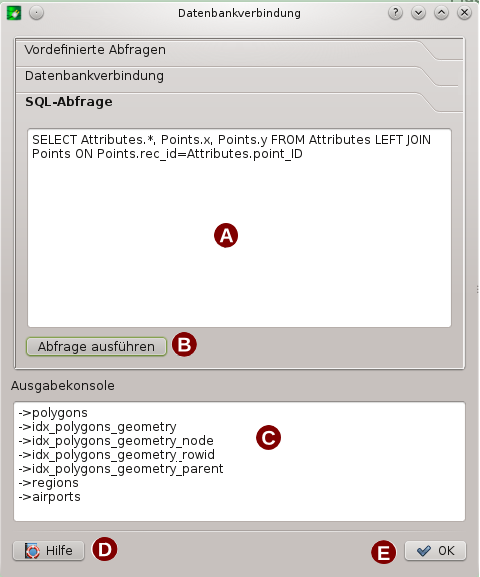
\includegraphics[clip=true, width=12cm]{evissql_query}
   \caption{Вкладка <<SQL-запрос>> расширения \emph{eVis} \wincaption}\label{evissql_query}
\end{figure}

\begin{itemize}[label=--]
\item \textbf{Текстовое поле SQL-запрос}: Место ввода SQL-запросов.
\item \textbf{Выполнить}: Кнопка выполнения SQL-запросов.
\item \textbf{Консоль вывода}: Консольное окно, в котором отображаются
сообщения, связанные с работой модуля.
\item \textbf{Справка}: Вызов окна справки.
\item \textbf{OK}: Закрыть главное окно \dialog{Соединение с БД}.
\end{itemize}

Используйте выпадающие меню \dropmenuopt{X-координата} и
\dropmenuopt{Y-координата} для выбора полей базы данных, в которых хранится
информация о координатах <<X>> (или долготе) и <<Y>> (или широте). После
нажатия кнопки OK на основе результатов SQL-запроса создаётся векторный
слой и добавляется в главное окно QGIS.

Чтобы сохранить векторный файл для будущего использования, примените
команду <<Сохранить как>>, доступную через правый щелчок на имени слоя в
списке слоёв QGIS.

\begin{Tip}\caption{\textsc{Создание векторного слоя на основе данных
листа Microsoft Excel}} При создании векторного слоя из листа Microsoft
Excel могут появиться строки с нежелательными нулями (<<0>>), вставленные
в таблицу атрибутов после корректных данных. Причиной может быть удаление
значений этих ячеек в Excel клавишей <<backspace>>. Для исправления проблемы
необходимо открыть файл Excel (предварительно закрыв QGIS, если данный файл
открыт на редактирование) и, используя инструмент Edit > Delete, удалить
пустые строки из файла. Во избежании такой проблемы, перед сохранением
файла следует просто удалять пустые строки в Excel, используя инструмент
Edit > Delete.
\end{Tip}

\minisec{Запуск предопределённых запросов}\label{evis_predefined}

С помощью инструмента предопределённых запросов можно загружать заранее
подготовленные запросы, хранящиеся в файле формата XML. Это особенно удобно
в случае, если вы не знакомы с командами SQL. Для этого необходимо перейти
во вкладку \tab{Предопределённые запросы}.

Чтобы загрузить набор предопределённых запросов, нажмите кнопку
\toolbtntwo{evis_file}{Открыть файл}. Появится окно, предназначенное для
определения расположения файла, содержащего SQL запросы. Когда запросы будут
загружены, их заголовки согласно определению в XML-файле появятся в выпадающем
списке, расположенном чуть ниже кнопки \toolbtntwo{evis_file}{Открыть файл},
полное описание выбранного запроса отобразится в текстовом поле, расположенном
под выпадающим списком.

Из выпадающего списка выберите запрос, который вы хотите запустить, и перейдите
во вкладку \tab{SQL-запрос}, чтобы просмотреть детали запроса. Убедитесь, что
соединение с базой данных установлено.

Для выполнения запроса во вкладке \tab{SQL-запрос} нажмите кнопку
\button{Выполнить}. Если запрос успешен, то появится окно \dialog{Выбор файла~БД}.
Если запрос некорректный, то в консоли вывода появится сообщение об ошибке.

\begin{figure}[htp]
   \centering
   
\includegraphics[clip=true, width=10cm]{evispredefined}
   \caption{Вкладка <<Предопределённые запросы>> расширения \emph{eVis} \wincaption}\label{evispredefined}
\end{figure}

\begin{itemize}[label=--]
\item \textbf{Открыть файл}: Вызов окна <<Открыть файл>> для поиска
XML-файла, содержащего предопределённые запросы.
\item \textbf{Предопределённые запросы}: Выпадающий список, содержащий запросы,
определённые в XML-файле.
\item \textbf{Описание запроса}: Короткое описание запроса, берётся из
XML-файла.
\item \textbf{Консоль вывода}: Консольное окно, в котором отображаются
сообщения, связанные с работой модуля.
\item \textbf{Справка}: Вызов окна справки.
\item \textbf{OK}: Закрыть главное окно \dialog{Соединение с БД}.
\end{itemize}

\minisec{XML-формат предопределённых запросов eVis}\label{evis_xml_format}

\begin{table}[htp]\index{модули!eVis}
\centering
 \begin{tabular}{|p{1.2in}|p{4.7in}|}
 \hline \textbf{Тег} & \textbf{Описание}\\
 \hline query & Определяет начало и конец запроса.\\
 \hline shortdescription & Короткое описание запроса, появляющееся в
 выпадающем меню eVis.\\
 \hline description & Более детальное описание запроса, отображается в
 текстовом поле вкладки <<Предопределённые запросы>>.\\
 \hline databasetype & Тип базы данных, соответствует выбору типа в
 выпадающем списке <<Тип соединения>> вкладки \tab{Соединение с БД}.\\
 \hline databaseport & Порт, соответствует определению порта в текстовом поле
 <<Порт вкладки>> \tab{Соединение с БД}.\\
 \hline databasename & Имя базы данных, соответствует определению имени базы
 данных в текстовом поле <<База данных>> вкладки \tab{Соединение с БД}.\\
 \hline databaseusername & Имя пользователя базы данных, соответствует
 определению имени пользователя в текстовом поле <<Пользователь>> вкладки
 \tab{Соединение с~БД}.\\
 \hline databasepassword & Пароль базы данных, соответствует определению
 пароля в текстовом поле <<Пароль>> вкладки \tab{Соединение с БД}.\\
 \hline sqlstatement & SQL-комманда.\\
 \hline autoconnect & Флаг (<<true>> или <<false>>) для определения, должны ли
 вышеуказанные параметры автоматически использоваться для подключения к базе
 данных без запуска процедуры соединения через вкладку \tab{Соединение с БД}.\\
 \hline
\end{tabular}
\caption{XML-теги eVis}\label{tab:evis_xml_tags}\medskip
\end{table}

Пример XML-файла, содержащего три запроса:

\begin{verbatim}
<?xml version="1.0"?>
<doc>
 <query>
   <shortdescription>Import all photograph points</shortdescription>
   <description>This command will import all of the data in the SQLite database to QGIS
      </description>
   <databasetype>SQLITE</databasetype>
   <databasehost />
   <databaseport />
   <databasename>C:\textbackslash Workshop/textbackslash
eVis\_Data\textbackslash PhotoPoints.db</databasename>
   <databaseusername />
   <databasepassword />
   <sqlstatement>SELECT Attributes.*, Points.x, Points.y FROM Attributes LEFT JOIN
      Points ON Points.rec_id=Attributes.point_ID</sqlstatement>
   <autoconnect>false</autoconnect>
 </query>
  <query>
   <shortdescription>Import photograph points "looking across Valley"</shortdescription>
   <description>This command will import only points that have photographs "looking across
      a valley" to QGIS</description>
   <databasetype>SQLITE</databasetype>
   <databasehost />
   <databaseport />
   <databasename>C:\Workshop\eVis_Data\PhotoPoints.db</databasename>
   <databaseusername />
   <databasepassword />
   <sqlstatement>SELECT Attributes.*, Points.x, Points.y FROM Attributes LEFT JOIN
      Points ON Points.rec_id=Attributes.point_ID where COMMENTS='Looking across
      valley'</sqlstatement>
   <autoconnect>false</autoconnect>
 </query>
 <query>
   <shortdescription>Import photograph points that mention "limestone"</shortdescription>
   <description>This command will import only points that have photographs that mention
      "limestone" to QGIS</description>
   <databasetype>SQLITE</databasetype>
   <databasehost />
   <databaseport />
   <databasename>C:\Workshop\eVis_Data\PhotoPoints.db</databasename>
   <databaseusername />
   <databasepassword />
   <sqlstatement>SELECT Attributes.*, Points.x, Points.y FROM Attributes LEFT JOIN
      Points ON Points.rec_id=Attributes.point_ID where COMMENTS like '%limestone%'
      </sqlstatement>
   <autoconnect>false</autoconnect>
 </query>
</doc>
\end{verbatim}

\FloatBarrier
